\documentclass{ifacmtg}
\bibliographystyle{ifac}
\usepackage{graphicx}


\begin{document}
\runauthor{Oswald et.al.}
\begin{frontmatter}
\title{Antenna calibration of the STEREO/WAVES antennas in the frequency range of the fixed frequency receiver}
\author[iwf]{T.H. Oswald}
\author[iwf]{W. Macher}
\author[iwf]{H.O. Rucker}
\author[iowa]{G. Fischer}
\author[iwf]{U. Taubenschuss}
\author[med]{J.L. Bougeret}
\author[med]{A. Lecacheux}
\author[green]{M.L. Kaiser}
\author[min]{K.Goetz}


\address[iwf]{Space Research Institute, Austrian Academy of Sciences, Graz, Austria}
\address[iowa]{University of Iowa, USA}
\address[med]{Observatoire de Paris-Meudon, France}
\address[green]{NASA/GSFC, Greenbelt, MD, USA}
\address[min]{University of Minnesota, USA}

\begin{abstract}
The STEREO/WAVES experiment includes a fixed frequency receiver which operates at the frequencies of 30.025 MHz and 32.025 Mhz which is well outside the quasi-static range. For this reason, the antenna calibration has to be performed separately at these frequencies and the results have to be treated with special care with regard to the sensitivity on changes of frequency and direction of incidence. The results of these calibrations shall be presented in this paper.
\end{abstract}

\begin{keyword}
STEREO, SWAVES, antennas, antenna calibration
\end{keyword}
\end{frontmatter}

\section{Introduction}
In October 2006 NASA has launched the two STEREO spacecraft with the radio
experiment SWAVES on board, designed to observe
solar radio emissions. The
STEREO-WAVES (SWAVES) experiment is designed to track solar and
interplanetary radio bursts and trace the generation and evolution
of radio disturbances from the Sun to the Earth orbit and beyond.
Each spacecraft has three, nearly orthogonal, antennas, capable of
receiving electromagnetic waves in several frequency ranges. While the
main operation range of the receivers is between 10kHz and 16MHz, there is additionally a fixed frequency receiver (FFR) on board which operates in the frequency range of 30.025 MHz and 32.025 Mhz. These higher frequencies enable a comparison between space-based and earth-based observations.

For the correct interpretation of the produced data it is of vital importance to know the antenna properties with great accuracy. The antenna properties of a receiving antenna can be described in a very concise manner by use of the effective length vector, or by computing the radiation pattern. Additionally the antenna impedance, which is closely related to the length of the effective length vector, is a very useful quantity to know.

The antennas will be directed away from the sun, so that they remain out of view of the sunward looking instruments on the spacecraft. Since the surface spacecraft hull and the solar panels are made of conducting material it has an appreciable effect on the antenna properties.

There are several possible methods in use for the calibration of spacecraft antennas.

\begin{itemize}
    \item The numerical method
\item Rheometry
\item EMC chamber
\item In-flight calibration\end{itemize}

At the Space Research Institute we perform the numerical method, and rheometry. Rheometry gives the quasistatic solution and is not applicable at the frequencies of the FFR. Hence this article deals only with the numerical method of calibrating the spacecraft antennas.


\subsection{The spacecraft and the SWAVES experiment}
The spacecraft and mission are described in detail in \cite{oswald07}, where the results of the STEREO antenna calibration are presented for the frequency range up to 16MHz, as well as \cite{bale07}. Therefore these items will only be described very briefly here. The STEREO/WAVES experiment works with three mutually orthogonal
monopole antennas. They are connected to several receivers. One of these receivers is the fixed frequency receiver (FFR) which operates only at the two frequencies at approximately 30MHz, which where mentioned above. To deal with the calculations of antenna properties at this frequency requires slightly different considerations which will be demonstrated in section \ref{sec:representation}.

\subsection{The coordinate frame}

\begin{figure}
\includegraphics[width=7.6cm]{PaperPics2/coordinate_system.eps}
\caption{The coordinate frame}
\label{fig_coord_frame}
\end{figure}

The reference frame used in this article is defined in a way to be spacecraft fixed with the positive x-axis in a direction which will point to the sun during most of the time, so the antennas are mounted on the side of the hull which points to the negative x-axis. The solar panels point to the positive and negative y-axis and the z-axis is defined to complete the right handed cartesian frame (Figure \ref{fig_coord_frame}).

For the description of the direction of the antennas we chose to use a spherical polar system which has the positive x-axis as polar axis. The angle $\zeta$ is the angle between the positive x-axis and the antenna, and $\xi$ is the azimuthal angle around the x-axis.

The boom points to the negative x-axis. There are 3 orthogonal monopole antennas, which are called $E_x$, $E_y$ and $E_z$, each 6 meters long. They are directed about $125.26^\circ$ from the x-axis and the difference in azimuth is $120^\circ$. The azimuth of antenna $E_z$ defines the azimuth of $0^\circ$. It is expected, that the boom has an effect to push the 3 electrical antennas away from the boom's position. This effect is increased by the high gain antenna, which is located near the boom. The panels are expected to push the effective length vectors towards the negative x-axis.

The antennas will be directed away from the sun, so that they remain out of view of the sunward looking instruments on the spacecraft.

\subsection{The representation of a transmitting and receiving antenna}\label{sec:representation}
A highly useful concept for representing the property of a receiving antenna is the effective length
vector which can be represented concisely by using a transfer matrix. The effective length vector represents the antenna as it behaves electrically in contrast to how it is built physically. It can deviate in direction and length from the physical antenna. The reason is the complicated body of the spacecraft which is electromagnetically coupled to the antenna and therefore has to be regarded as part of the antenna system itself. The effective length vector is a complex vector depending on frequency and direction of incidence of the received wave. Only at the quasistatic limit the imaginary part tends to zero and the directional dependance vanishes but this is not true for the frequencies of the FFR. Hence the concept of the effective length vector is not useful to represent the properties of the antennas at the FFR frequencies.

Another method to represent antenna properties, which seems more appropriate for describing antenna properties in this frequency range is the power pattern. Patterns, a widely used concept in antenna theory, are three dimensional plots of a field quantity as function of direction. In case of the power pattern the magnitude of the Poynting vector as function of the frequency is plotted. Often the normalized power pattern is used.

\begin{equation}\label{power_pattern}
    P(\theta,\phi)=\frac{|\mathbf{S}(\theta,\phi)|}{|\mathbf{S}(\theta,\phi)_{max}|}
\end{equation}

P is the relative gain and S is the Poynting vector which represents the energy flux per square meter per second. The Poynting vector can be computed as

\begin{equation}\label{poynting_vector}
    \mathbf{S}(\theta,\phi)=(\mathbf{e}_{\theta} \times \mathbf{e}_{\phi}) \frac{E_{\theta}^2+E_{\phi}^2}{\eta}
\end{equation}

$\mathbf{e}_{\theta}$ and $\mathbf{e}_{\phi}$ are the unit vectors in $\theta$ and $\phi$ direction and $\eta$ is the impedance of free space.

\begin{figure}
\hrule
%\vspace*{8cm}
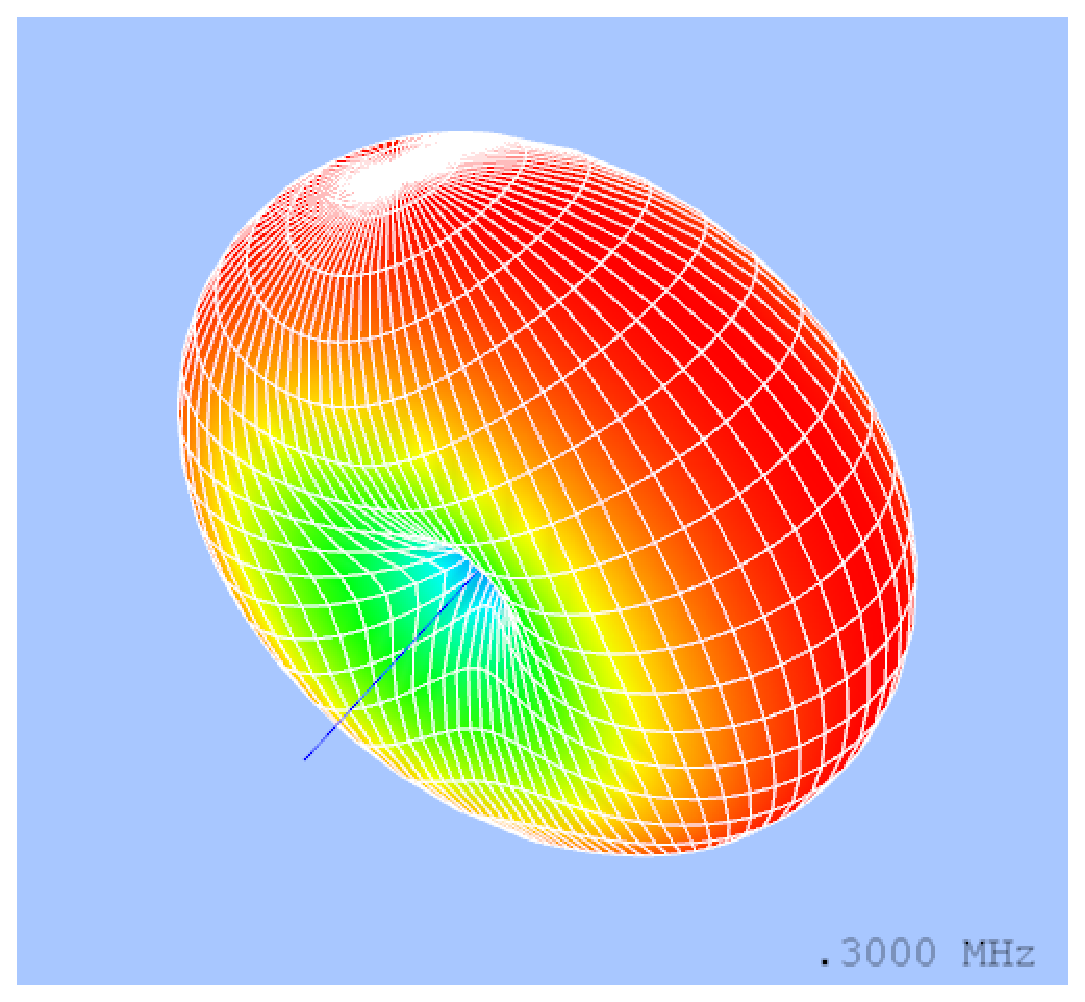
\includegraphics[width=7.6cm]{PaperPics2/dipole_pattern.eps}
%\vbox to 8cm{\vfill \hbox to \hsize{\hfill  \hfill}\vfill}
\hrule
\caption{Power pattern of a dipole}
\label{fig_dipole_pattern}
\end{figure}

\begin{figure}
\hrule
%\vspace*{8cm}
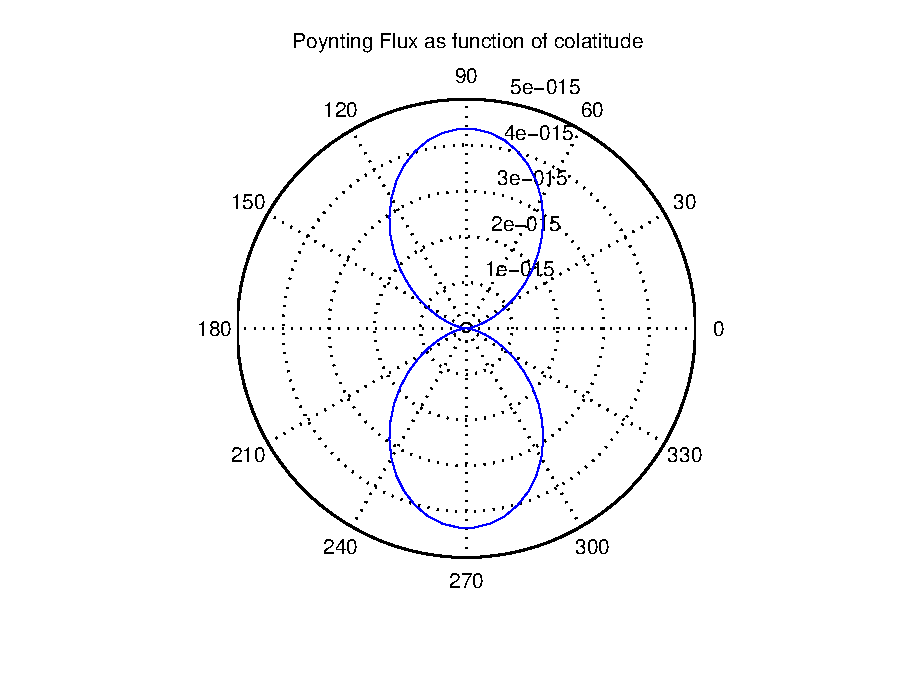
\includegraphics[width=7.6cm]{PaperPics2/dipole_2d.eps}
%\vbox to 8cm{\vfill \hbox to \hsize{\hfill  \hfill}\vfill}
\hrule
\caption{Projection of the power pattern of a dipole}
\label{fig_dipole_pattern_2d}
\end{figure}

In symmetrical systems it is often useful to plot the projection of the power pattern as function of just one of the coordinates. Figure \ref{fig_dipole_pattern} shows the 3D power pattern of a dipole which has the characteristic toroidal shape, while figure \ref{fig_dipole_pattern_2d} shows the 2D counterpart which shows the gain as function of the colatitude.

An other important property of an antenna is the antenna impedance. It can be seen as the complex resistance of the antenna element in a circuit diagram. The real part is often called the antenna resistance and is a measure of the sensitivity of the antenna. Therefore it is proportional to the length of the effective vector. The real part tends to zero, while the imaginary part tends to minus infinity in the quasistatic limit. In this range the antenna behaves purely capacitively.

At the frequency where the imaginary part of the antenna impedance crosses the zero axis, the antenna resonates. At the resonance frequency the antenna is purely resistive. This is typically the case at the frequency where distance between the tip of the effective length vector and the furthest part of the spacecraft body corresponds to a multiple of a half wavelength. Near this frequency the antenna is very sensitive but the effective length vectors behave erratically. Thus the antenna behavior is hard to determine in this range.

The impedances of the spacecraft antennas can be represented by the impedance matrix. Figure \ref{fig:impedances} shows a diagram of the real and imaginary part of the impedances. The frequencies of the FFR are outside the range of the influence of a resonance. Nevertheless the resistance does not vanish as in the quasistatic case and has to be taken into account. Contrary to the quasistatic case, the capacitance matrix can not be used instead of the impedance matrix to describe the antenna behavior. Additionally a complicated dependance of the effective length vectors on frequency and direction can be expected.


\begin{figure}
\hrule
%\vspace*{8cm}
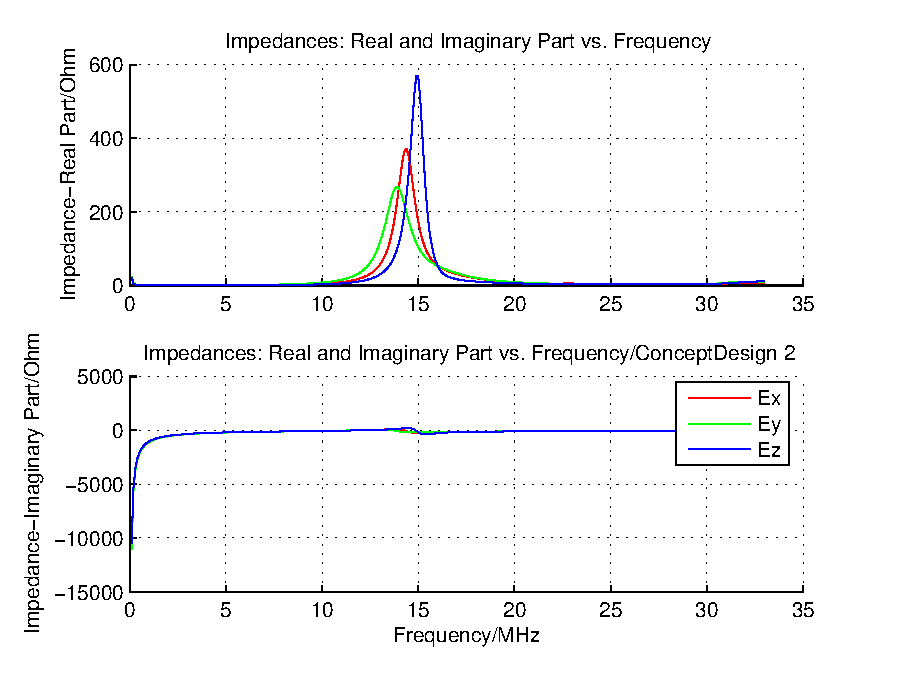
\includegraphics[width=7.6cm]{PaperPics2/impedance.eps}
%\vbox to 8cm{\vfill \hbox to \hsize{\hfill  \hfill}\vfill}
\hrule
\caption{Real and imaginary part of the impedances of the SWAVES antennas.}
\label{fig:impedances}
\end{figure}


\begin{figure}
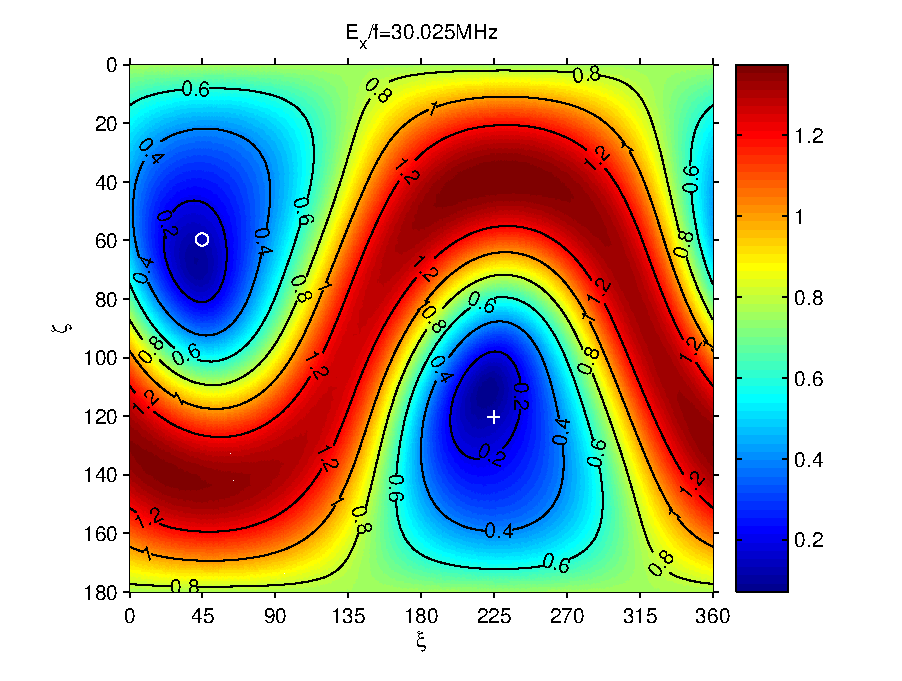
\includegraphics[width=7.6cm]{PaperPics2/deviationf1.eps}
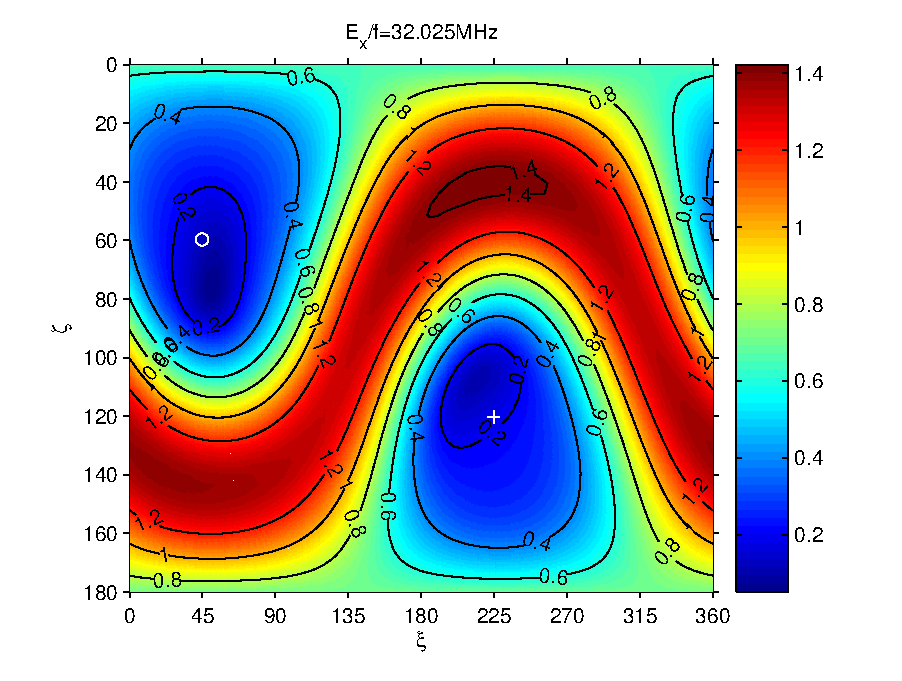
\includegraphics[width=7.6cm]{PaperPics2/deviationf2.eps}
\caption{Deviation of the perpendicular component of the effective length vector of the x-antenna from the quasi-static case at the frequencies of the FFR}
\label{fig:deviation}
\end{figure}

Figures \ref{fig:deviation} show the relative deviation of the perpendicular component, i.e. perpendicular to the incident wave, of the effective length vector to the constant effective length vector in the quasi-static limit as a function of direction of incidence. The surfaces show a quite complicated pattern, and the relative difference has a maximum of $140\%$. The small white cross is placed at the direction of the quasi-static effective length vector, while the small circle indicates the opposite direction.

\begin{figure}
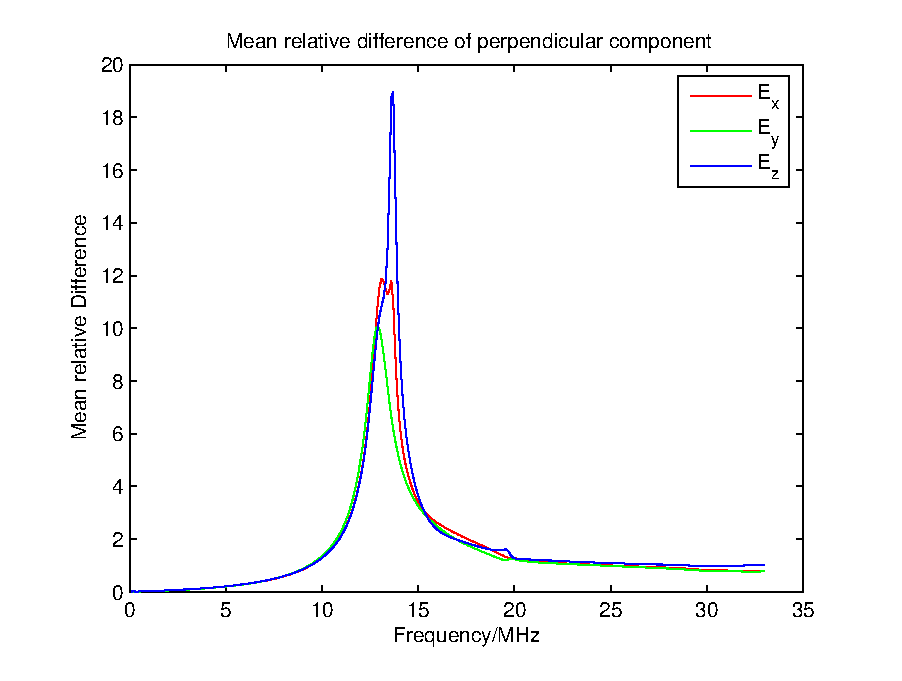
\includegraphics[width=7.6cm]{PaperPics2/meandev.eps}
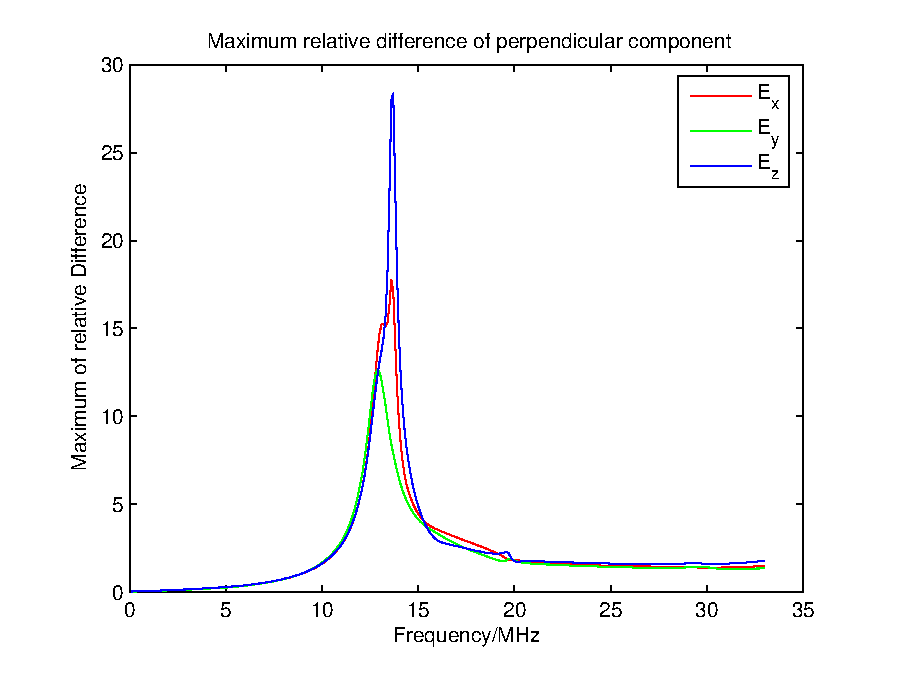
\includegraphics[width=7.6cm]{PaperPics2/maxdev.eps}
\caption{Mean and maximum of the perpendicular components of the effective length vectors of the antennas from the quasi-static case as a function of frequency}
\label{fig:meanmaxdev}
\end{figure}

Figures \ref{fig:meanmaxdev} show the mean and maximum of the perpendicular components of the effective length vectors of the antennas from the quasi-static case at a given frequency as a function of frequency. By comparing figures \ref{fig:impedances} with \ref{fig:meanmaxdev} it can clearly be seen that the frequency range with the highest variability of the effective length vectors is identical to the frequency range surrounding the resonance. While the frequencies of the FFR are not close to the resonance frequency, the variability is too high to be neglected.

\section{The numerical method}
Two steps are required to calculate the antenna parameters mentioned in the last section. First the current distribution along the surface of the spacecraft has to be computed. Usually it is not possible to find an analytic solution for this kind of problem, except for some very simple problems which show a very symmetric geometry. Therefore one has to resort to numerical procedures to determine a solution. For this purpose the spacecraft can be modeled of simple basic elements which can be rods or patches, i.e. flat triangles or quadrangles.

Once the currents are known the parameters describing the behavior of the spacecraft-antenna-system can be calculated. For the computation of the currents, two different software packages were used, a modified version of an open source program called antenna scatterers analysis program (ASAP) originally written by J.H.�Richmond at the Ohio State University, extended by J.W.� McCormack at the Naval Postgraduate School, and a proprietary software package called CONCEPT II, written at the the University of Hamburg-Harburg.

The computation of the relevant antenna parameters where performed by using Matlab routines. The points important for understanding the relevance of the results of the parameters at the frequencies of the FFR will be summarized in the following two sections.


\subsection{Calculation of the current distribution}
Both software packages, ASAP and CONCEPT II use simple building blocks to model the geometry of the spacecraft. ASAP uses rods while CONCEPT can deal with rods and/or patches, which are small flat triangles or quadrangles. The size of the basic elements must be small in relation to the wavelength used, which is a restriction easily fulfilled when dealing with the frequencies of the FFR. The corresponding wavelengths are about 10m. An additional restriction is the relation between the largest and the smallest element, which must not be too large. This and the computing time limit the amount of detail which can accurately be modeled. A high detail level as it is possible when using experimental procedures is, at this time, not possible when using numerical methods.

Even though the programs use different representations of the spacecraft, as well as different equations, the resulting parameters describing the antenna behavior must agree. The consistency of the two results is a good indication for the validity of the method and the modeling process. The final test is the consistency with experimental methods and the ability to reproduce actual measurements once the spacecraft are in their operating stage.

In order to calculate the current distribution along the surface of a conducting body, the corresponding field integral has to be set up and solved in combination with the correct boundary conditions. ASAP uses the reaction integral equation (RIE), while CONCEPT uses the electric field integral equation (EFIE) for the rods and a combination of EFIE and the magnetic field integral equation (MFIE) for models which include rods and patches.

Each antenna is excited by a source of 1V located at the feed, which is located near the point where the antenna touches the spacecraft body. The source can either be a point source or be distributed along a rod. ASAP can deal with both cases, while CONCEPT always locates the feed at one point inside one of the rods.

The integral is solved numerically by using the method of moments (MOM) \cite{harrington}. It is converted into a matrix equation and solved by means of linear algebra. Hereby the currents along each wire are represented as the sum of a set of weighed base functions. ASAP uses two sinusoidal functions as base function, while CONCEPT uses the sum of up to eight triangular base functions for rods and roof functions to describe the current distribution on the surface of a patch.

The RIE used by ASAP uses the reciprocity principle. It has the advantage that it considers also magnetic currents as sources and is therefore ending up with a symmetric matrix. This symmetry can be used to accelerate the computation. In contrast to the EFIE, it models the currents flowing on the surface of the rods. Using this method it is easier to include rods made of dielectric materials. Since the currents are not real but virtual, the method gives correct solutions in the quasistatic range where the EFIE would break down because in reality the currents at low frequencies would be located not only at the surface, but also inside the material. One would have to take care about this fact when using the EFIE, while the equivalent currents resulting from the RIE methods are set up in away such that this effect is included automatically.

The EFIE is a more direct approach, easier to understand and derive.

Using patches, the actual current distribution can be modeled with more accuracy which is important with increasing frequency. The magnetic field integral equation is used to compute the currents on the surface of the patches. Rods have to be used additionally in order to represent structures like the antennas, so the resulting system of equations comprises both types of equations. A disadvantage is that the computation time increases dramatically. Nevertheless the results at the frequencies of the FFR are expected to be most accurate when using patches, this will be the method of choice when computing the corresponding currents. Only CONCEPT can deal with models made of patches.

Details about the RIE can be found in \cite{momentmethods}, while the methods used in CONCEPT are described very accurately in \cite{concept}. Figures \ref{fig:grids} show the wire-grid and the patch model we used for our calculations.

\begin{figure}
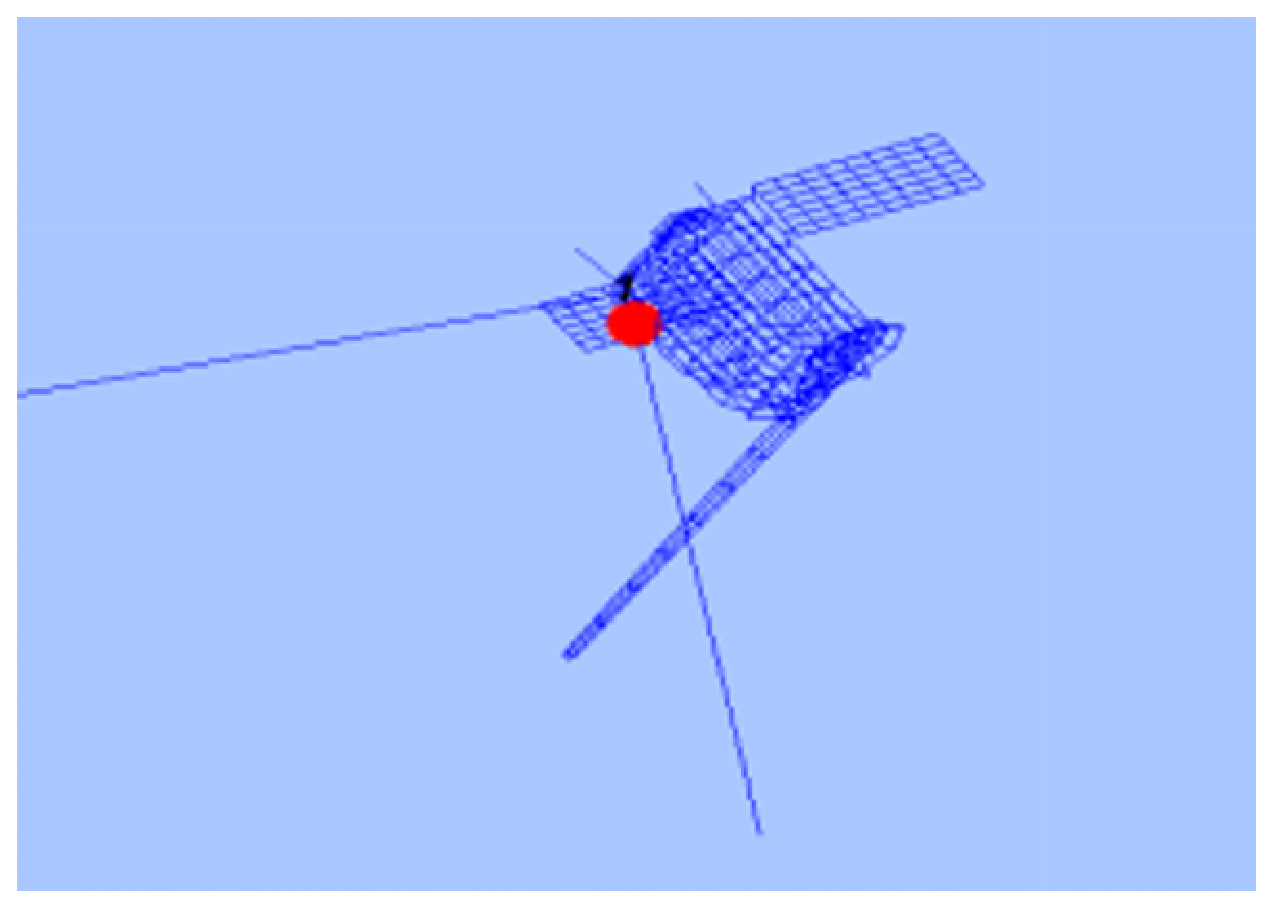
\includegraphics[width=7.6cm]{PaperPics2/wiregrid.eps}
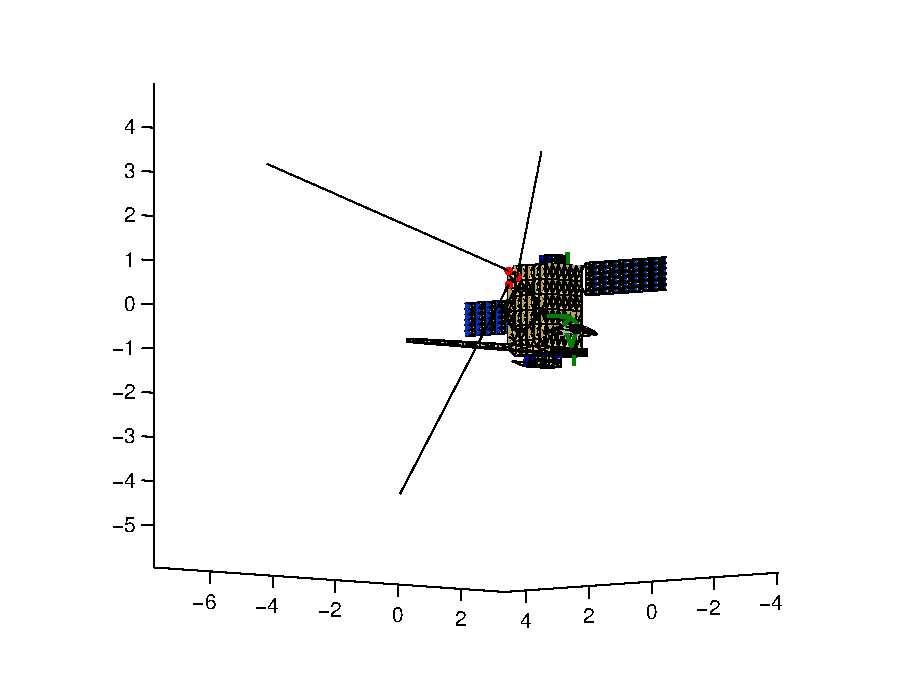
\includegraphics[width=7.6cm]{PaperPics2/patchgrid.eps}
\caption{Wire-grid and patch-grid model}
\label{fig:grids}
\end{figure}

\subsection{Further calculations}
Once the currents are known, all other antenna parameters can be calculated, which was done by using Matlab. The calculation was done for open feeds and for loaded feeds where the total base capacitance  (receiver, cable and antenna mounting) was estimated to be 90pF, which has to be taken parallel to the antenna capacitance in the case of the transmitting antenna, while it is in series at the receiving antenna.

The effective length vector can be calculated from the current distribution by using the equation

\begin{equation}\label{get_heff}
    \mathbf{h}_{eff} = \frac{1}{I_0} \int \mathbf{J} (\mathbf{r}) e^{- \imath \mathbf{k} \cdot \mathbf{r}}d\mathbf{r}'
\end{equation}

$I_0$ is the current at the feed. Details can be found in
\cite{macher_dipl}.

The input impedance can be computed by dividing the voltage at the feed by the current.

The power pattern can be computed in two different ways, simulating a transmitting or a receiving antenna.

\begin{itemize}
    \item Using the transmitting antenna, the radiated far field is computed as a function of direction. This can be achieved by integration the currents along all wires or over the while surface of the spacecraft. From the far field, the poynting flux can be computed, which is proportional to the power pattern.
    \item The receiving antenna method uses the concept of the effective length vector. The component of the effective length vector in the direction perpendicular to the direction of the incident electromagnetic wave is a proportional the the magnitude of the power pattern in a given direction. For a constant effective length vector this method always yields a pattern of toroidal shape, but since the direction and length of the effective length vector depends on the direction quite strongly at the frequencies of the FFR, the shape of the power pattern could be quite irregular.
\end{itemize}



\section{The results of the determination of the effective length vectors of the STEREO/WAVES antennas}
\subsection{Introduction}
Numerical calculations, using ASAP and the ASAP toolbox, to determine the characteristics of the three antennas of the STEREO/SWAVES experiment were performed. Such calculations were done fore the Cassini spacecraft \cite{cassini}, \cite{cassini2} and \cite{vogl_01} as well as Mars Express \cite{marsis} and \cite{marsis2} and other spacecraft in the past. A summary can be found in \cite{ruckerundi05}.

\subsection{The spacecraft characteristics}

%\begin{figure}
%\hrule
%\includegraphics[width=7.6cm]{PaperPics/stereo1.eps}
%\hrule
%\caption{The STEREO spacecraft}
%\label{stereo1}
%\end{figure}

One characteristic of the STEREO spacecraft is a certain degree of asymmetry (Figure \ref{stereo1}). In contrast to many other spacecraft, the solar panels are positioned at different longitudinal distances at the spacecraft hull. Additionally the spacecraft consist of an about 6 meters long boom, and a turnable high gain antenna. These prominent features will have an influence on the antenna characteristics. The boom is divided into 4 sections with different diameters and has great influence upon the effective length vectors of the antennas.


The two spacecraft, A and B are almost identical, apart of some small differences of their instrumentation. The only difference which can be modeled within the limitations of the algorithm is the second ring, mounted on the hull of spacecraft B on the positive x side, and not existent on spacecraft A.


The model of the Stereo spacecraft consist of the following parts:

\begin{enumerate}
\item The hull
\item 2 solar panels
\item The high gain antenna
\item Three 6 meter long antennas
\item A 6 meter long boom
\item A ring mounted on the hull of spacecraft A, two rings on spacecraft B\\
\end{enumerate}

%\begin{figure}
%\hrule
%%\vspace*{8cm}
%\includegraphics[width=7.6cm]{PaperPics/stereo_model.eps}
%%\vbox to 8cm{\vfill \hbox to \hsize{\hfill  \hfill}\vfill}
%\hrule
%\caption{The stereo model}
%\label{fig_stereo_model}
%\end{figure}

Size and position of the parts were measured from the relevant construction plans. The part of the tapered boom which is near to the spacecraft hull is modeled as prism with triangular base. Figure \ref{fig_stereo_model} shows the model from an oblique view.
%
\subsection{The determination of the effective length vectors at the quasistatic limit}
As a first step the currents at frequencies from 100 kHz to 34 MHz were calculated by using ASAP and CONCEPT II in turn. The frequency spacing was 100 kHz. Using this data, the impedances, admittances and effective length vectors were computed with our matlab routines. The direction of the incident wave was taken to be the positive x-axis, simulating radiation from the sun.

Meanwhile the rheometry measurements were performed. A correction for the real antenna diameter had to be applied for the rheometry and the results which were obtained by use of ASAP. The CONCEPT II software allows different diameters of individual segments, so we could take the antenna diameters into account directly.

\begin{table}[htbp]
\caption{STEREO A, open feeds at 300kHz} \label{tab_heff1}
\begin{tabular*}{\hsize}{lllll}
\hline
 &  & ASAP & CONCEPT II & Physical \\
 & & & & antennas\\
\hline
 & length/m & 2.30 & 2.34 & 6.00 \\
  E1 & $\zeta$/$^\circ$ & 133.7& 133.5 & 125.3\\
& $\xi$/$^\circ$ & 21.4 & 21.5 & 0.0\\
\hline
& length/m & 3.82 & 3.88  & 6.00\\
  E2 & $\zeta$/$^\circ$ & 119.1 & 118.6 & 125.3\\
& $\xi$/$^\circ$ & 129.3 & 129.2  & 120.0\\
\hline
& length/m & 3.03 & 3.07 & 6.00\\
  E3 & $\zeta$/$^\circ$ & 126.0 & 125.6  & 125.3\\
& $\xi$/$^\circ$ & -141.6 & -141.6  & -120.0 \\
\hline
\end{tabular*}
\end{table}

\begin{table}[htbp]
\caption{STEREO A, open feeds at 300kHz} \label{tab_heff2}
\begin{tabular*}{\hsize}{lllll}
\hline
 &  & ASAP & Rheometry & Physical \\
& & & & antennas\\
\hline
 & length/m & 2.30  & 2.36 & 6.00 \\
  E1 & $\zeta$/$^\circ$ & 133.7 & 132.2 & 125.3\\
& $\xi$/$^\circ$ & 21.4  & 21.6 & 0.0\\
\hline
& length/m & 3.82  & 3.84 & 6.00\\
  E2 & $\zeta$/$^\circ$ & 119.1  & 118.7 & 125.3\\
& $\xi$/$^\circ$ & 129.3  & 127.9 & 120.0\\
\hline
& length/m & 3.03  & 2.89 & 6.00\\
  E3 & $\zeta$/$^\circ$ & 126.0  & 126.2 & 125.3\\
& $\xi$/$^\circ$ & -141.6  & -140.7 & -120.0 \\
\hline
\end{tabular*}
\end{table}

\begin{table}
\caption{STEREO A, loaded feeds at 300kHz}
\label{tab_heff3}
\begin{tabular*}{\hsize}{lllll}
\hline
 &  & ASAP & CONCEPT II & Physical\\
& & & & antennas\\
\hline
 & length/m & 0.96 & 0.96  & 6.00 \\
  E1 & $\zeta$/$^\circ$ & 124.9& 123.9  & 125.3\\
& $\xi$/$^\circ$ & 15.4 & 15.0 & 0.0\\
\hline
& length/m & 1.43 & 1.42  & 6.00\\
  E2 & $\zeta$/$^\circ$ & 114.7  &113.9  & 125.3\\
& $\xi$/$^\circ$ & 127.5 & 127.3  & 120.0\\
\hline
& length/m & 1.19 & 1.17  & 6.00\\
  E3 & $\zeta$/$^\circ$ & 120.3 & 119.3  & 125.3\\
& $\xi$/$^\circ$ & -135.3 & -134.8  & -120.0 \\
\hline
\end{tabular*}
\end{table}

The result of the calculations can be seen in tables \ref{tab_heff1} and \ref{tab_heff2} for open feeds ant in table \ref{tab_heff3} for base capacitances of 90pF. The frequency is 300kHz which is well in the quasistatic limit. For comparison, the lengths and orientation information of the physical antennas are also added.

The quasistatic results are in full concurrence with our expectations. All electric antennas have lengths which are shorter than half the length of the physical antennas, as expected by theory for monopole antennas that are small in relation to the wavelength. The influence of the capacitances on the effective length vectors seems to be quite substantial. A similar calculation without taking the capacitances into account resulted in effective length vectors which were approximately half the length of the physical antennas. Furthermore, it can clearly be seen that the solar panels push the electric antennas towards the negative x-axis with a counteracting influence of the boom. The results of the numerical and experimental determination are very consistent.

\subsection{Variation of the properties with frequency and direction}

As mentioned before, direction finding is only possible in the lower frequency regions. At higher frequencies, the effective length vectors become complex and dependent on frequency and direction of incidence.

%\begin{figure}
%\hrule
%%\vspace*{8cm}
%\includegraphics[width=7.6cm]{PaperPics/HeffLengthAbsD3.eps}
%%\vbox to 8cm{\vfill \hbox to \hsize{\hfill  \hfill}\vfill}
%\hrule
%\caption{Magnitude of the effective length vector as function of frequency}
%\label{fig_hefflength_abs}
%\end{figure}


Figure \ref{fig_hefflength_abs} shows the magnitude of the effective length vector as function of frequency, where this behavior can easily be spotted. The direction of incidence was taken to be the x axis which corresponds to the direction of the sun. Between 20 and 25MHz there is a resonance which occurs when the distance between the tips of the effective length vectors is in a special relation to the wavelength of the incident wave. When the antenna resonates, its response to the radiation is very high which corresponds to a large effective length vector.

%\begin{figure}
%\hrule
%%\vspace*{8cm}
%\includegraphics[width=7.6cm]{PaperPics/var_dir_300khz_A1.eps}
%%\vbox to 8cm{\vfill \hbox to \hsize{\hfill  \hfill}\vfill}
%\hrule
%\caption{Magnitude of the effective length vector as function of direction of incidence at 300kHz}
%\label{fig_var_dir_300k}
%\end{figure}
%
%\begin{figure}
%\hrule
%%\vspace*{8cm}
%\includegraphics[width=7.6cm]{PaperPics/var_dir_10Mhz_A1.eps}
%%\vbox to 8cm{\vfill \hbox to \hsize{\hfill  \hfill}\vfill}
%\hrule
%\caption{Magnitude of the effective length vector as function of direction of incidence at 10MHz}
%\label{fig_var_dir_10m}
%\end{figure}


Figures \ref{fig_var_dir_300k} and \ref{fig_var_dir_10m} show the magnitude of the effective length vector of antenna 1 as function of the direction of incidence at 300kHz and 10MHz respectively, using open feeds. The variability at 300kHz is negligible which is not true at 10MHz. This has to be taken into account when data at high frequencies is analyzed.

When direction finding is regarded to be possible with the knowledge of the directions of the electric antennas with an accuracy of 2 degrees, further analysis dictate an upper limit of not more than 2MHz where direction finding can be done by using standard methods. Fortunately figure \ref{fig_var_dir_10m} suggest that even at higher frequencies and in the region near the resonance frequency, the effective length vectors behave in a predictable manner, i.e. they are not chaotic. Further analysis shows that the function is also continuous regarding frequency variations.

\subsection{Variation of the effective length vectors with different HGA orientations}
The high gain antenna (HGA) on the STEREO spacecraft is mounted turnable (figure \ref{fig_hga}) We investigated the effect of HGA orientation on the effective length vectors.

%\begin{figure}
%\hrule
%%\vspace*{8cm}
%\includegraphics[width=7.6cm]{PaperPics/hga_positions_D3.eps}
%%\vbox to 8cm{\vfill \hbox to \hsize{\hfill  \hfill}\vfill}
%\hrule
%\caption{The turnable high gain antenna}
%\label{fig_hga}
%\end{figure}

Analysis of the influence of the orientation of the HGA upon the effective length vectors has shown that the deviation is, in general, irrelevant. As an example figures \ref{fig_var_HGA_300k} and \ref{fig_var_dir_10m} show the magnitude of the effective length vectors as function of the angle od the HGA with open feeds at 300kHz and 10MHz respectively.


%\begin{figure}
%\hrule
%%\vspace*{8cm}
%\includegraphics[width=7.6cm]{PaperPics/var_hga_length_300khz.eps}
%%\vbox to 8cm{\vfill \hbox to \hsize{\hfill  \hfill}\vfill}
%\hrule
%\caption{Magnitude of the effective length vector as function of HGA angle at 300kHz}
%\label{fig_var_HGA_300k}
%\end{figure}
%
%\begin{figure}
%\hrule
%%\vspace*{8cm}
%\includegraphics[width=7.6cm]{PaperPics/var_hga_length_10mhz.eps}
%%\vbox to 8cm{\vfill \hbox to \hsize{\hfill  \hfill}\vfill}
%\hrule
%\caption{Magnitude of the effective length vector as function of HGA angle at 10MHz}
%\label{fig_var_HGA_10m}
%\end{figure}

\subsection{The impedances and capacitances}
Figures \ref{fig_imp_open} and \ref{fig_imp_loaded} show the antenna impedances for the STEREO antennas in 2 different representations. The results of the first figure were calculated with open feeds, for the second figure loaded feeds were used. At the frequency where the imaginary part is zero, the first resonance is located. At this frequency the impedance is pure resistive. The inclusion of the capacitances of the receiver, the cable and the antenna mounting has the effect to decrease the resonance frequency. When regarding the case of transmitting antennas, the base capacitances are parallel to the antenna capacitances and both can be added. To get the overall impedance, the reciprocal values have to be added, while the admittances have simply to be added.





\section{Conclusion}
In this paper four different methods of spacecraft antenna calibration were described. Some results of the two methods which have already been performed on the Space Research Institute for the STEREO spacecraft were given to demonstrate the consistency of the situation.

It is of vital importance that several possible methods are performed for each antenna system to be studied. Either method has its own advantages. Rheometry can be far more detailed than it would be possible for the wire-grid simulations, so the influence of the fine structure of the spacecraft can be estimated by comparison of the two methods. Rheometry is therefore a good basis to decide about improvements of wire-grids, it further yields a purely quasi-static result, which must agree with the asymptotic limit of the numeric calculations as the frequency converges to zero. The advantage of the computer simulation is the flexibility regarding the model structure, so it can be used to study the perturbation of antenna properties provoked by single spacecraft parts. Of course, the decisive advantage is that electromagnetic codes are devised for high-frequency analysis up to frequencies far above the resonance, thereby enabling the estimation of the validity range of the quasi-static results.

Figure \ref{fig_freq_range} show the frequency ranges of the receivers of some spacecraft which where calibrated at our institute, as well as the frequency ranges where the methods are valid. Fortunately the larger part of the frequency range of interest is at low frequencies where rheometry and the numerical method are valid. Therefor we can use both methods to compliment and validate each other as was demonstrated in this paper.




\
\bibliography{../../Bibliography/MyBib}

\end{document}
